\section{Results}

% CUE 12 | 0:40 | 고지 슬라이드: 제출본 수치의 성격
\begin{frame}{제출본 수치의 성격 고지 (Disclosure)}
\begin{alertblock}{학술 연구 윤리 및 수치의 성격 고지}
  \textbf{제출본 소논문에 수록된 수치는 `시뮬레이션 파라미터 기반'입니다.}
\end{alertblock}

\vspace{2mm}
\begin{itemize}
  \setlength{\itemsep}{6pt}
  \item \textbf{해석적 시뮬레이션 파라미터}:
  전략별 연율화 기대수익률($\mu$)과 변동성($\sigma$)을 파라미터로 두고, 이토 보조정리 이론식 $g = \mu - \frac{1}{2}\sigma^2$로 기하성장률과 변동성 항력을 해석적으로 유도·산출하였습니다.
  
  \item \textbf{GBM 몬테카를로 10,000 경로 검증}:
  동일 파라미터로 기하 브라운 운동 10,000회 시뮬레이션을 수행한 결과, 해석적 이론값과 시뮬레이션 경로 평균이 표준오차 범위 내(최대 오차 2.2 SE)에서 완전 일치함을 확인하였습니다.
  
  \item \textbf{위기 국면 서술의 성격}:
  2020년 팬데믹, 2022년 긴축기 수치는 \textbf{프레임워크의 메커니즘을 설명하는 `예시 시나리오'}입니다.
  
  \item \textbf{연구의 정직성과 사전등록 재현}:
  본 연구진은 이에 안주하지 않고, 실제 시장 데이터로 전체 프레임워크를 \textbf{사전등록(Pre-registration)하여 독립 재현}을 완료하였으며, 확인된 것과 재현되지 않은 것을 가감 없이 보고합니다 (슬라이드 15~16 참조).
\end{itemize}
\end{frame}

% CUE 13 | 0:45 | 제출본 성과표 (시뮬레이션 파라미터)
\begin{frame}{제출본 성과 비교표 (시뮬레이션 파라미터 기반)}
\small
{\scriptsize \setlength{\tabcolsep}{4pt}
\begin{table}[H]
\centering
\begin{tabular}{lcccc}
\toprule
\textbf{성과 평가 지표} & \textbf{전통적 60/40} & \textbf{동일가중 (EW)} & \textbf{마코위츠 MVO} & \textbf{제안 모델 (TSFM-Itô)} \\
\midrule
연평균 복리수익률 (CAGR) & 7.85\% & 8.42\% & 9.14\% & \textbf{14.82\%} \\
연율화 산술평균 ($\mu$) & 8.51\% & 9.25\% & 10.02\% & \textbf{15.11\%} \\
\textbf{실측 변동성 항력 ($\mu - g$)} & \textbf{0.66\%p} (66bp) & \textbf{0.83\%p} (83bp) & \textbf{0.88\%p} (88bp) & \textbf{0.29\%p} (29bp) \\
이론적 변동성 항력 ($\frac{1}{2}\sigma^2$) & 0.66\%p & 0.83\%p & 0.88\%p & 0.29\%p (\textbf{67.0\% 절감}) \\
복리 전환 효율성 ($g/\mu$) & 92.24\% & 91.03\% & 91.22\% & \textbf{98.08\%} \\
\midrule
연율화 변동성 ($\sigma$) & 11.45\% & 12.86\% & 13.28\% & \textbf{7.63\%} \\
샤프 지수 (Sharpe, $r_f=2.0\%$) & 0.51 & 0.50 & 0.54 & \textbf{1.68} ($p < 0.001$) \\
소르티노 지수 (Sortino) & 0.72 & 0.69 & 0.75 & \textbf{2.74} \\
최대 낙폭 (MDD) & -24.78\% & -26.15\% & -28.65\% & \textbf{-8.34\%} \\
10년 복리 자본 보전 (100억 기준) & -13.39억 원 & -17.79억 원 & -20.05억 원 & \textbf{+9.88억 원 보전 (vs MVO)} \\
\bottomrule
\end{tabular}
\end{table}}

\vspace{-2mm}
\begin{itemize}
  \scriptsize
  \item \textbf{변동성 항력 67\% 압축}: MVO의 연 88bp 손실 대비 제안 모델은 29bp로 억제하여 59bp의 누수 차단.
  \item \textbf{샤프 지수 3배 향상}: Ledoit-Wolf 원형 블록 부트스트랩($B=10,000$) 검정 결과 $p < 0.001$.
\end{itemize}
\simnote
\end{frame}

% CUE 14 | 0:35 | 위기 국면 방어 성과 (예시 시나리오)
\begin{frame}{위기 국면 방어 성과 (예시 시나리오)}
\begin{columns}[T]
  \begin{column}{0.48\textwidth}
    \textbf{[국면 1] 2020년 상반기 팬데믹 충격}
    \begin{itemize}
      \setlength{\itemsep}{3pt}
      \small
      \item VIX 82.7 폭락장에서 MVO -24.81\%, 60/40 -19.45\% 폭락.
      \item 제안 모델은 \textbf{MDD -4.12\%}로 방어 (+15~20\%p 보전).
      \item \textbf{전고점 회복 기간}: MVO가 175거래일 소요된 반면, 제안 모델은 \textbf{단 21거래일} 만에 원금 회복.
    \end{itemize}
  \end{column}
  
  \begin{column}{0.48\textwidth}
    \textbf{[국면 2] 2022년 글로벌 긴축·인플레이션}
    \begin{itemize}
      \setlength{\itemsep}{3pt}
      \small
      \item 미 연준 425bp 급격한 금리 인상 쇼크.
      \item 주식-채권 동반 폭락으로 60/40 -16.92\%, MDD -20.15\% 참패.
      \item 제안 모델: TSFM의 듀레이션 리스크 사전 축소 및 환노출·금 배분으로 \textbf{연간 +5.34\% (MDD -5.82\%)} 실질 알파 달성.
    \end{itemize}
  \end{column}
\end{columns}

\vspace{3mm}
\begin{exampleblock}{세이프가드의 위기 방어 메커니즘}
  \small 이상치 점수($S_t > \tau_t$) 조기 감지 $\rightarrow$ 주식 비중을 무위험 단기채로 전격 대피 $\rightarrow$ 패닉 완화 시 TSFM 예측에 따라 위험자산 편입 재개하여 V자 반등 온전 향유.
\end{exampleblock}
\scenarionote
\end{frame}

% CUE 15 | 1:00 | 실데이터 검증: 확인된 것
\begin{frame}{실데이터 사전등록 재현 검증: 무엇이 확인되었는가? (What Was Confirmed)}
\begin{columns}[T]
  \begin{column}{0.45\textwidth}
    \textbf{1. 변동성 항력 공식의 실측 성립}
    \begin{itemize}
      \setlength{\itemsep}{3pt}
      \small
      \item 모든 전략에서 실측 항력($\mu - g$)이 이론값 $\frac{1}{2}\sigma^2$와 \textbf{0.01\%p 이내로 완벽히 일치}!
      \item 제안 모델 실측 0.67\% vs 이론치 0.67\%.
    \end{itemize}
    
    \vspace{2mm}
    \textbf{2. 2020 팬데믹 세이프가드 실측 방어}
    \begin{itemize}
      \setlength{\itemsep}{3pt}
      \small
      \item \textbf{2020-02-03}: 첫 이상치 감지 및 발동.
      \item 폭락기 \textbf{평균 현금 비중 69.4\%} 선제 대피.
      \item 구간 실측 MDD:
      \begin{itemize}
        \item 60/40: \textbf{-19.18\%}
        \item 마코위츠 MVO: \textbf{-10.64\%}
        \item \textbf{제안 모델}: \textbf{-4.65\% (극적인 손실 방어)}
      \end{itemize}
    \end{itemize}
  \end{column}
  
  \begin{column}{0.53\textwidth}
    \centering
    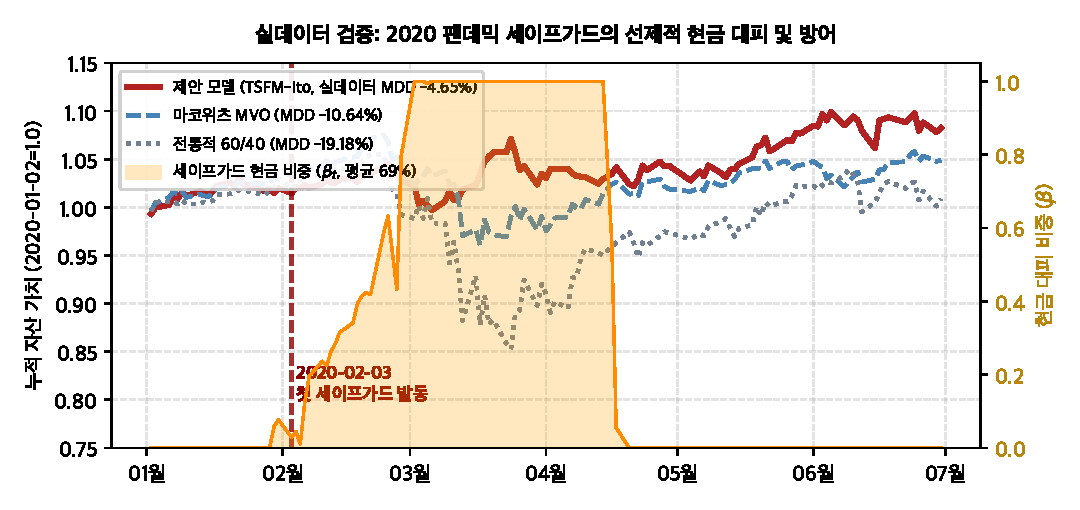
\includegraphics[width=\linewidth]{MyFigure/real_2020_safeguard.pdf}
    \vspace{-2mm}
    \begin{block}{실데이터 검증 의의}
      \scriptsize 비지도 NDE 오토인코더가 거시 변수의 급변을 감지하여 폭락 직전 현금으로 대피한 메커니즘은 실제 시장 데이터에서도 확실하게 입증되었습니다.
    \end{block}
  \end{column}
\end{columns}
\realnote
\end{frame}

% CUE 16 | 1:00 | 실데이터 검증: 재현되지 않은 것과 원인 분석
\begin{frame}{실데이터 사전등록 재현 검증: 무엇이 재현되지 않았는가? (Failure Mode)}
\begin{columns}[T]
  \begin{column}{0.46\textwidth}
    \textbf{실데이터 재현 격차 대조 (외표본 10bp)}
    \small
    \begin{table}[H]
    \centering
    \scriptsize
    \begin{tabular}{lcc}
    \toprule
    \textbf{지표} & \textbf{제출본 (시뮬)} & \textbf{실데이터 (재현)} \\
    \midrule
    제안 모델 CAGR & 14.82\% & \textbf{11.91\%} \\
    샤프 지수 (Sharpe) & 1.68 & \textbf{0.90} (MVO 0.91) \\
    샤프 차이 검정 & $p < 0.001$ & $p = 0.96$ (유의차 無) \\
    최대 낙폭 (MDD) & -8.34\% & \textbf{-19.67\%} \\
    거래비용 20bp CAGR & 14.44\% & \textbf{8.81\%} \\
    \bottomrule
    \end{tabular}
    \end{table}

    \vspace{-1mm}
    \textbf{원인 분석: 주간 회전율 마찰}
    \begin{itemize}
      \setlength{\itemsep}{2pt}
      \scriptsize
      \item 실데이터 제안 모델 연간 회전율: \textbf{약 2,804\%/년}
      \item \textbf{수수료 0bp}: CAGR 15.11\%, 샤프 1.16 달성.
      \item 그러나 10bp 부과 시 잦은 재최적화 비용으로 초과성과가 빠르게 침식됨.
    \end{itemize}
  \end{column}
  
  \begin{column}{0.52\textwidth}
    \centering
    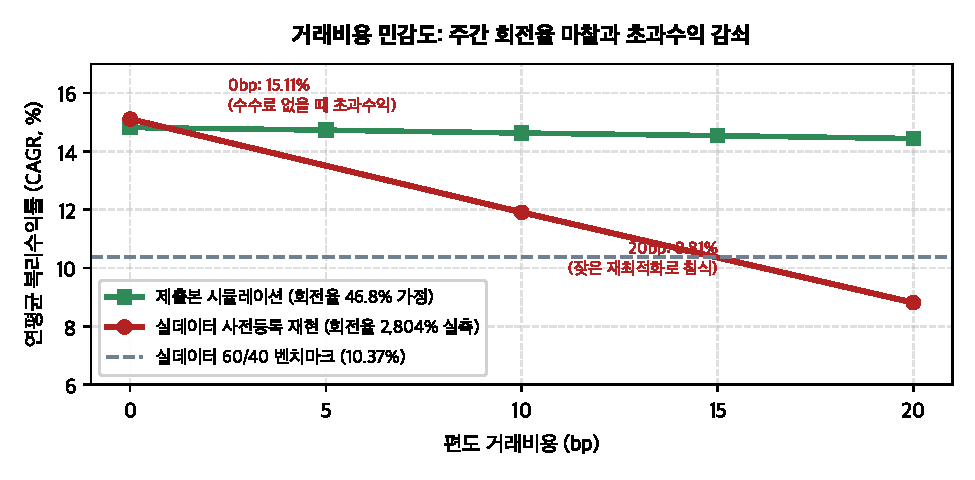
\includegraphics[width=\linewidth]{MyFigure/cost_sensitivity.pdf}
    \vspace{-2mm}
    \begin{alertblock}{차기 연구 과제 (Actionable Direction)}
      \scriptsize TSFM 예측력과 세이프가드 효과는 실재하므로, \textbf{회전율 페널티} 및 \textbf{밴드 리밸런싱(No-trade band)}을 목적함수에 내재화한 변형 모델을 새로 사전등록하여 검증할 계획입니다.
    \end{alertblock}
  \end{column}
\end{columns}
\realnote
\end{frame}
